\chapter{Latent Factor Topic Modelling | Text clustering}

% \begin{figure}[h]
%    {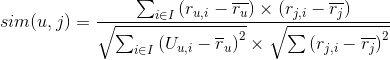
\includegraphics[scale=1]{img/PearsonEqn.png}}
% \end{figure}
Topic Modelling has been a way to comprehend text for the machine learning community. This can be of supervised or unsupervised nature. For the task of this thesis, we have employed the unsupervised version of the topic modelling. A number of simple unsupervised methods can be used for feature selection in text clustering. Some examples of such methods are discussed below.

\section{Document Frequency-based Selection}
The simplest possible method for feature selection in document clustering is that of the use of document frequency to filter out irrelevant features. While the use of inverse document frequencies reduces the importance of such words, this may not alone be sufficient to reduce the noise effects of very frequent words. In other words, words which are too frequent in the corpus can be removed because they are typically common words such as “a”, “an”, “the”, or “of” which are not discriminative from a clustering perspective. Such words are also referred to as stop words.
A variety of methods are commonly available in the literature [76] for stop-word removal.  Typically commonly available stop word lists of
about 300 to 400 words are used for the retrieval process. In addition,
words which occur extremely infrequently can also be removed from
the collection. This is because such words do not add anything to the
similarity computations which are used in most clustering methods. In some cases, such words may be misspellings or typographical errors in
documents. Noisy text collections which are derived from the web, blogs
or social networks are more likely to contain such terms. We note that
some lines of research define document frequency based selection purely
on the basis of very infrequent terms, because these terms contribute the
least to the similarity calculations. However, it should be emphasized
that very frequent words should also be removed, especially if they are
not discriminative between clusters. Note that the TF-IDF weighting
method can also naturally filter out very common words in a “soft” way.
Clearly, the standard set of stop words provide a valid set of words to
prune. There are other ways of quantifying the important words directly to the clustering process, which is essential to more aggressive pruning.

\section{Term Strength}
A much more aggressive technique for stop-word removal has been p





